\section{Elaborazione statistico-probabilistica delle piogge intense della stazione di riferimento per il bacino in esame (analisi degli afflussi)}
In questo capitolo della relazione si condurrà un'analisi statistico-probabilistica degli eventi pluviometrici del bacino. In particolare, si utilizzerà la distribuzione di probabilità dei valori estremi (legge di Gumbel).\\
Successivamente, verrà effettuata la verifica dell'adattamento della serie di valori pluviometrici alla distribuzione, facendo ricorso al test di Matalas.\\
Infine, si svolgeranno i calcoli per determinare la Linea Segnalatrice di Possibilità Pluviometrica (LSPP).\\
Essendo che si andrà a svolgere i calcoli considerando solamente i massimi annuali di precipitazione, occorre che tali valori debbano: 
\begin{itemize}
    \item essere relativi ad un certo periodo di tempo (almeno 30 anni);
    \item essere \textit{casuali, omogenei, indipendenti e stazionari}.
\end{itemize} 
In particolare, essendo la procedura di calcolo uguale per ogni serie numerica, verrà svolta la spiegazione per la durata pluviometrica di 30 minuti, per poi riportare solamente i risultati.

\subsection{Verifica preliminare visiva  (mediante \textit{Plotting position} e distribuzione delle classi)}
\label{sec_plotting_position}
Prima di svolgere l'adattamento della serie pluviometrica misurata a quella degli estremi di Gumbel, occorre valutare se tali valori si adattano correttamente lungo la retta di distribuzione teorica.\\
Ad ogni misura della serie, posta in ordine crescente, viene attribuito un valore a seconda della propria posizione nel campione, secondo il metodo di Weibull $(P_{em}= \frac{i}{N+1})$ o Hazen $\left(P_{em}=\frac{i-0.5}{N}\right)$. Entrambi questi parametri correlano l'evento di precipitazione con la probabilità di non superamento dell'evento (anche indicato come $P$).\\
Utilizzando il valore ricavato da uno di questi metodi, viene calcolata una variabile d'appoggio ($y$), secondo la formula $y = -ln(-ln(P))$, essendo che $P(x)= e ^{-e^ {-y}}$.\\
Successivamente, utilizzando i parametri $y$ (appena calcolato), $\alpha$ e $u$, quest'ultimi basati sul campione, si riesce a ricavare l'altezza di precipitazione dell'evento, regolarizzata secondo la distribuzione di Gumbel, secondo la formula inversa di $y = \alpha (h - u)$.
\begin{equation}
    \alpha = \left(\frac{1.283}{\sigma(h)}\right)
\end{equation}
\begin{equation}
    u = \left( h_m - \frac{0.5772}{\alpha} \right)
\end{equation}
\begin{equation}
    h = \frac{y}{\alpha}+u
    \label{eq:h_tr}
\end{equation}
Al fine di verificare visivamente la bontà degli allineamenti delle distribuzioni della serie osservata e della serie attesa (teorica), occorre creare un grafico dove, in ascissa si pone il valore del parametro $y$ ed in ordinata si pongono i valori delle relative precipitazioni teoriche. I grafici sono riportati nel successivo capitoletto.\\
Maggiore è l'allineamento tra le due distribuzioni e migliore sarà la distribuzione della serie osservata.\\
Inoltre, per valutare preliminarmente la serie, può essere utile suddividere le precipitazioni per classi omogenee (per vedere come si distribuiscono i valori all'interno di esse) e calcolare i principali parametri statistici.

\begin{table}[H] \centering
    \caption{\textcolor{red}{Valori di probabilità di non superamento dell'evento (calcolata mediante Weibull e Hazen) e relativo valore del parametro d'appoggio $y$, riferito ad una durata di precipitazione di 0.5 ore.}}
    \begin{tabular}{cccccc}
 &  & \multicolumn{2}{c}{\textbf{Plotting Position}} & \multicolumn{2}{c}{\textbf{Y -ln( -ln (1- 1/Tr))}}\\
 \toprule
    \textbf{n} & \textbf{h [mm] 0.5 ore} & \textbf{P Weibull   n/N+1} & \textbf{P Hazen  (n-0,5)/N} & \textbf{y Weibull} & \textbf{y Hazen}\\
\midrule
    1          & 11.2                        & 0.026                      & 0.014                       & -1.291                  & -1.460                  \\
    2          & 12                          & 0.053                      & 0.041                       & -1.080                  & -1.165                  \\
    3          & 12.2                        & 0.079                      & 0.068                       & -0.932                  & -0.991                  \\
    4          & 12.6                        & 0.105                      & 0.095                       & -0.812                  & -0.858                  \\
    5          & 13.8                        & 0.132                      & 0.122                       & -0.707                  & -0.745                  \\
    6          & 14.2                        & 0.158                      & 0.149                       & -0.613                  & -0.645                  \\
    7          & 15                          & 0.184                      & 0.176                       & -0.526                  & -0.553                  \\
    8          & 16                          & 0.211                      & 0.203                       & -0.443                  & -0.468                  \\
    9          & 16.4                        & 0.237                      & 0.230                       & -0.365                  & -0.386                  \\
    10         & 16.6                        & 0.263                      & 0.257                       & -0.289                  & -0.307                  \\
    11         & 17.2                        & 0.289                      & 0.284                       & -0.215                  & -0.231                  \\
    12         & 17.4                        & 0.316                      & 0.311                       & -0.142                  & -0.156                  \\
    13         & 17.4                        & 0.342                      & 0.338                       & -0.070                  & -0.082                  \\
    14         & 18                          & 0.368                      & 0.365                       & 0.001                   & -0.008                  \\
    15         & 18                          & 0.395                      & 0.392                       & 0.073                   & 0.065                   \\
    16         & 18.6                        & 0.421                      & 0.419                       & 0.145                   & 0.139                   \\
    17         & 19                          & 0.447                      & 0.446                       & 0.218                   & 0.214                   \\
    18         & 19.6                        & 0.474                      & 0.473                       & 0.291                   & 0.289                   \\
    19         & 20                          & 0.500                      & 0.500                       & 0.367                   & 0.367                   \\
    20         & 20.2                        & 0.526                      & 0.527                       & 0.443                   & 0.446                   \\
    21         & 20.4                        & 0.553                      & 0.554                       & 0.522                   & 0.527                   \\
    22         & 21                          & 0.579                      & 0.581                       & 0.604                   & 0.611                   \\
    23         & 22.4                        & 0.605                      & 0.608                       & 0.689                   & 0.698                   \\
    24         & 22.6                        & 0.632                      & 0.635                       & 0.778                   & 0.790                   \\
    25         & 22.6                        & 0.658                      & 0.662                       & 0.871                   & 0.886                   \\
    26         & 23.4                        & 0.684                      & 0.689                       & 0.969                   & 0.988                   \\
    27         & 25.6                        & 0.711                      & 0.716                       & 1.074                   & 1.097                   \\
    28         & 25.6                        & 0.737                      & 0.743                       & 1.186                   & 1.215                   \\
    29         & 25.8                        & 0.763                      & 0.770                       & 1.308                   & 1.343                   \\
    30         & 26.6                        & 0.789                      & 0.797                       & 1.442                   & 1.485                   \\
    31         & 27                          & 0.816                      & 0.824                       & 1.592                   & 1.644                   \\
    32         & 27                          & 0.842                      & 0.851                       & 1.761                   & 1.827                   \\
    33         & 27.8                        & 0.868                      & 0.878                       & 1.958                   & 2.043                   \\
    34         & 27.8                        & 0.895                      & 0.905                       & 2.196                   & 2.309                   \\
    35         & 29.4                        & 0.921                      & 0.932                       & 2.498                   & 2.660                   \\
    36         & 32.6                        & 0.947                      & 0.959                       & 2.918                   & 3.185                   \\
    37         & 38.4                        & 0.974                      & 0.986                       & 3.624                   & 4.297         \\
    \bottomrule         
    \end{tabular}
    \label{table:prec_05ore}
    \end{table}

\begin{table}[H] \centering
    \caption{\textcolor{red}{Principali parametri statistici riferiti alla serie pluviometrica di durata 0.5 ore.}}
 \begin{tabular}{cc}
    \toprule
deviazione standard ($\sigma$) & 6.2  \\
media ($x_m$)              & 20.8 \\
$\alpha$            & 0.2  \\
$u$           & 18.1\\
N                & 37.0 \\
minimo ($x_{min}$)             & 11.2 \\
massimo ($x_{max}$)            & 38.4 \\
varianza ($\sigma^2$)             & 38.3 \\
coeff. variazione (CV)    & 0.30 \\
mediana ($x_{mediana}$)        & 20.0 \\
numero di classi (k)      & 5.5  \\
k scelto                 & 6.0  \\
verifica (Iman e Conover) & 64.0 \\
delta classe ($\Delta$)          & 4.5  \\
delta scelto             & 5.0 \\
        \bottomrule
        \end{tabular}
\end{table}    

La varianza ($\sigma ^2$) è un fattore che indica come i valori della serie si discostano dal quello medio (o da uno atteso).\\
La deviazione standard ($\sigma$), in modo simile alla variazione, indica la dispersione della serie numerica rispetto alla media; al contrario dell'indice statistico precedente, questo valore ha la stessa unità di misura della serie numerica, permettendo quindi il reciproco confronto.\\
Anche il coefficiente di variazione permette il confronto di fenomeni fisici o statistici aventi unità di misura differenti, essendo un parametro adimensionale.\\
La verifica di Iman e Conover ($2^k>N$) permette valutare se il numero di classi scelto per suddividere la serie è sufficientemente alto, per non averne un numero troppo basso e con un'alta densità di valori.\\
Il delta della classe ($\Delta$) indica la differenza tra il massimo valore della classe ed il minimo.

\begin{figure}[H]\centering
    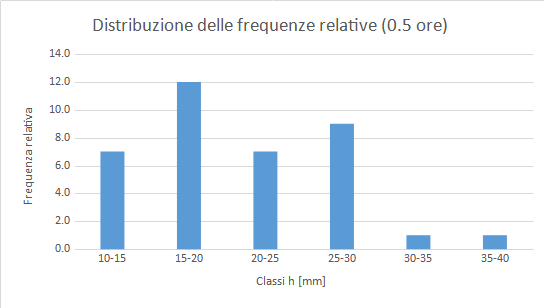
\includegraphics[scale=.6]{immagini/freq_piogg_rel_05ore.png}
    \caption{Distribuzione delle frequenze relative di pioggia (suddivise per classi omogenee), di un evento di durata 0.5 ore.}
  \label{freq_rel_piogg_05ore}
\end{figure}

\begin{figure}[H]\centering
    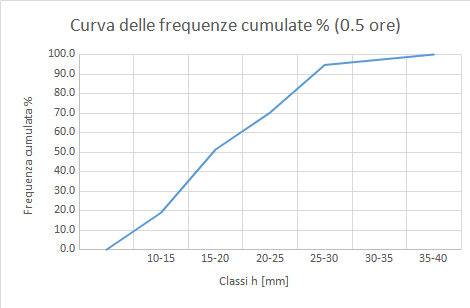
\includegraphics[scale=.6]{immagini/freq_piogg_cum_05ore.png}
    \caption{Frequenze di pioggia cumulata, relative ad un evento di durata 0.5 ore.}
  \label{freq_cum_piogg_05ore}
\end{figure}

\subsection{Calcolo delle altezze di pioggia per il $T_r$ di riferimento}
Successivamente ad aver verificato che l'allineamento tra le due distribuzioni è apprezzabile, occorre svolgere il calcolo delle altezze di pioggia, dati dei tempi di ritorno.\\
Essendo che $y = -ln(-ln(P))$ e $P = 1-\frac{1}{T_r}$, allora 
\begin{equation}
y = -ln\left(-ln\left(1-\frac{1}{T_r}\right)\right)
\end{equation}
Partendo da questo calcolo della variabile d'appoggio, è possibile ricavare l'altezza di precipitazione mediante \eqref{eq:h_tr}.

\begin{table}[H] \centering
    \caption{\textcolor{red}{Valori di altezza di pioggia attesa (teorica), calcolata mediante la variabile d'appoggio $y$ di Weibull o di Hazen (0.5 ore).}}
    \begin{tabular}{cccc}
 & & \multicolumn{2}{c}{$h = Y/\alpha + u$}       \\
 \toprule
    \textbf{n} & \textbf{h (mm)     0.5 ore} & \textbf{h mediante Weibull} & \textbf{h mediante Hazen} \\
\midrule
    1          & 11.2                        & 11.839                & 11.028                 \\
    2          & 12                          & 12.858                & 12.449                 \\
    3          & 12.2                        & 13.573                & 13.286                 \\
    4          & 12.6                        & 14.153                & 13.929                 \\
    5          & 13.8                        & 14.656                & 14.472                 \\
    6          & 14.2                        & 15.110                & 14.955                 \\
    7          & 15                          & 15.531                & 15.397                 \\
    8          & 16                          & 15.927                & 15.811                 \\
    9          & 16.4                        & 16.306                & 16.205                 \\
    10         & 16.6                        & 16.672                & 16.584                 \\
    11         & 17.2                        & 17.029                & 16.953                 \\
    12         & 17.4                        & 17.380                & 17.314                 \\
    13         & 17.4                        & 17.727                & 17.671                 \\
    14         & 18                          & 18.073                & 18.026                 \\
    15         & 18                          & 18.418                & 18.380                 \\
    16         & 18.6                        & 18.765                & 18.737                 \\
    17         & 19                          & 19.115                & 19.096                 \\
    18         & 19.6                        & 19.471                & 19.461                 \\
    19         & 20                          & 19.833                & 19.833                 \\
    20         & 20.2                        & 20.203                & 20.214                 \\
    21         & 20.4                        & 20.585                & 20.606                 \\
    22         & 21                          & 20.979                & 21.011                 \\
    23         & 22.4                        & 21.388                & 21.433                 \\
    24         & 22.6                        & 21.815                & 21.874                 \\
    25         & 22.6                        & 22.263                & 22.338                 \\
    26         & 23.4                        & 22.738                & 22.831                 \\
    27         & 25.6                        & 23.243                & 23.356                 \\
    28         & 25.6                        & 23.785                & 23.924                 \\
    29         & 25.8                        & 24.374                & 24.542                 \\
    30         & 26.6                        & 25.020                & 25.225                 \\
    31         & 27                          & 25.740                & 25.993                 \\
    32         & 27                          & 26.557                & 26.874                 \\
    33         & 27.8                        & 27.509                & 27.915                 \\
    34         & 27.8                        & 28.655                & 29.199                 \\
    35         & 29.4                        & 30.111                & 30.891                 \\
    36         & 32.6                        & 32.133                & 33.422                 \\
    37         & 38.4                        & 35.541                & 38.786          \\
    \bottomrule      
    \end{tabular}
    \end{table}

    \begin{figure}[H]\centering
        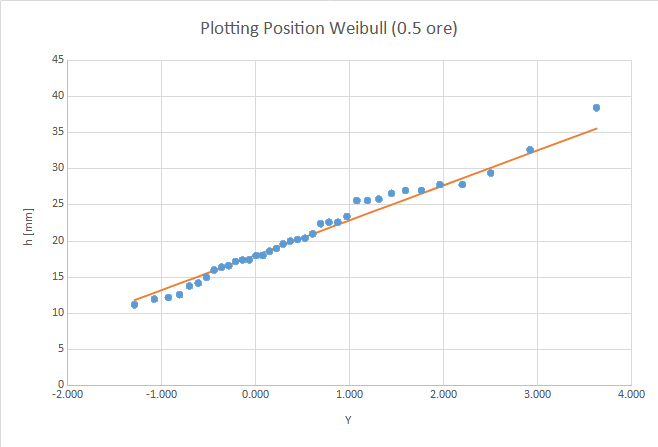
\includegraphics[scale=.5]{immagini/plot_pos_weib_05ore.png}
        \caption{Plotting position mediante weibull (0.5 ore).}
      \label{plot_pos_weib_05ore}
    \end{figure}

    \begin{figure}[H]\centering
        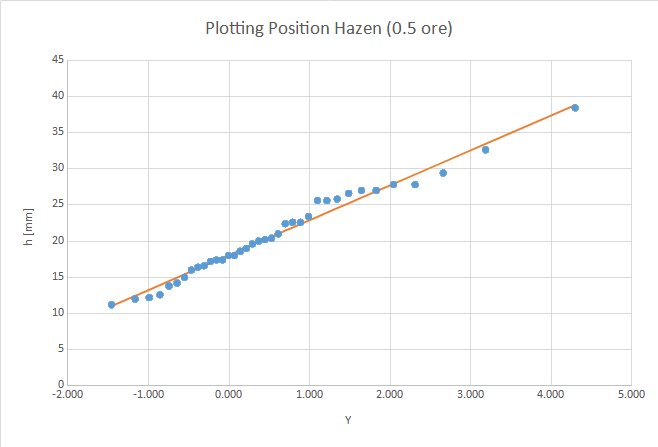
\includegraphics[scale=.5]{immagini/plot_pos_hazen_05ore.png}
        \caption{Plottin position mediante Hazen (0.5 ore).}
      \label{plot_pos_hazen_05ore}
    \end{figure}

\begin{table}[H] \centering
    \caption{\textcolor{red}{Altezze di pioggia attese per il $T_r$ di riferimento e durata di 0.5 ore.}}
        \begin{tabular}{ccc}
        \toprule
        Tr (anni) & y     & h attesa (mm) \\
        \midrule
        2 & 0.367 & 19.8  \\
        5 & 1.500 & 25.3  \\
        10  & 2.250 & 28.9          \\
        30  & 3.384 & 34.4          \\
        50  & 3.902 & 36.9          \\
        100 & 4.600 & 40.2          \\
        200 & 5.296 & 43.6          \\         
        \bottomrule
        \end{tabular}
\end{table}
    
\subsection{Test statistico di Matalas}
Similmente a come è stata svolta la verifica grafica (\ref{sec_plotting_position}), è necessario accertarsi che l'asimmetria ($G$) della serie osservata (storica) non differisca eccessivamente dalla serie teorica.\\
La procedura del test statistico è:
\begin{itemize}
\item calcolo del coefficiente di asimmetria $G$, mediante \eqref{eq:coef_asimmetria};
\item estrapolazione dei parametri $E(y)$ e $\sigma(y)$, in funzione di N;
\item verifica della disequazione \eqref{eq:disequazione_matalas}.
\end{itemize}
\begin{equation}
    G = \frac{m_3}{m_2^{\frac{3}{2}}} = N^{\frac{1}{2}} \frac{\sum_{i=1,N}(x_i - x_m)^3}{\left[\sum_{i=1,N}(x_i-x_m)^2\right]^{\frac{3}{2}}}
    \label{eq:coef_asimmetria}
\end{equation}
\begin{equation}
    |G - E (y)| < 2 \sigma(y)
    \label{eq:disequazione_matalas}
\end{equation}
Dove:
\begin{itemize}
    \item $G$: coefficiente di asimmetria del campione;
    \item $E(y)$: coefficiente di asimmetria del campione perfetto, che segue l'andamento di Gumbel;
    \item $\sigma (y)$: deviazione standard del campione.
\end{itemize}
Nel caso in cui la disequazione fosse corretta, è possibile accettare la distribuzione di probabilità di Gumbel. In caso contrario occorrerebbe provare un'altra distribuzione teorica di probabilità.

\begin{table}[H] \centering
    \caption{\textcolor{red}{Parametri per l'esecuzione del test statistico di Matalas, relativi alla durata di precipitazione di 0.5 ore.}}
    \begin{tabular}{cc}
    \toprule
    media                  & 20.85 \\
    $N ^{0.5}$ & 6.083 \\
    G                      & 0.622 \\
    G - E                  & 0.259 \\
    2 $\sigma$             & 1.069 \\
    TEST                   & Vero \\
    \bottomrule
    \end{tabular}
\end{table}

\subsection{Risultati delle altre durate di precipitazione}
Come anticipato precedentemente, in questa sezione vengono riportati solamente i risultati delle analisi matematiche (tabelle e grafici) per le altre durate di precipitazione.\\
I procedimenti per le seguenti durate sono i medesimi utilizzati per la durata di 0.5 ore.
\subsubsection{Durata di 1 ora}
\begin{table}[H] \centering
    \caption{\textcolor{red}{Valori di probabilità di non superamento dell'evento (calcolata mediante Weibull e Hazen) e relativo valore del parametro d'appoggio $y$, riferito ad una durata di precipitazione di 1 ora.}}
    \begin{tabular}{cccccc}
        &  & \multicolumn{2}{c}{\textbf{Plotting Position}} & \multicolumn{2}{c}{\textbf{Y -ln( -ln (1- 1/Tr))}}\\
        \toprule
           \textbf{n} & \textbf{h [mm] 1 ora} & \textbf{P Weibull   n/N+1} & \textbf{P Hazen  (n-0,5)/N} & \textbf{y Weibull} & \textbf{y Hazen}\\
       \midrule
    1          & 13.8                      & 0.026                      & 0.014                       & -1.291                  & -1.460                  \\
    2          & 14.4                      & 0.053                      & 0.041                       & -1.080                  & -1.165                  \\
    3          & 16.2                      & 0.079                      & 0.068                       & -0.932                  & -0.991                  \\
    4          & 17                        & 0.105                      & 0.095                       & -0.812                  & -0.858                  \\
    5          & 17.6                      & 0.132                      & 0.122                       & -0.707                  & -0.745                  \\
    6          & 17.8                      & 0.158                      & 0.149                       & -0.613                  & -0.645                  \\
    7          & 19.2                      & 0.184                      & 0.176                       & -0.526                  & -0.553                  \\
    8          & 19.4                      & 0.211                      & 0.203                       & -0.443                  & -0.468                  \\
    9          & 19.4                      & 0.237                      & 0.230                       & -0.365                  & -0.386                  \\
    10         & 20.6                      & 0.263                      & 0.257                       & -0.289                  & -0.307                  \\
    11         & 20.6                      & 0.289                      & 0.284                       & -0.215                  & -0.231                  \\
    12         & 21.2                      & 0.316                      & 0.311                       & -0.142                  & -0.156                  \\
    13         & 21.6                      & 0.342                      & 0.338                       & -0.070                  & -0.082                  \\
    14         & 21.8                      & 0.368                      & 0.365                       & 0.001                   & -0.008                  \\
    15         & 23.6                      & 0.395                      & 0.392                       & 0.073                   & 0.065                   \\
    16         & 23.6                      & 0.421                      & 0.419                       & 0.145                   & 0.139                   \\
    17         & 23.8                      & 0.447                      & 0.446                       & 0.218                   & 0.214                   \\
    18         & 24                        & 0.474                      & 0.473                       & 0.291                   & 0.289                   \\
    19         & 24.2                      & 0.500                      & 0.500                       & 0.367                   & 0.367                   \\
    20         & 24.4                      & 0.526                      & 0.527                       & 0.443                   & 0.446                   \\
    21         & 24.4                      & 0.553                      & 0.554                       & 0.522                   & 0.527                   \\
    22         & 24.8                      & 0.579                      & 0.581                       & 0.604                   & 0.611                   \\
    23         & 25.8                      & 0.605                      & 0.608                       & 0.689                   & 0.698                   \\
    24         & 26.8                      & 0.632                      & 0.635                       & 0.778                   & 0.790                   \\
    25         & 27                        & 0.658                      & 0.662                       & 0.871                   & 0.886                   \\
    26         & 27.6                      & 0.684                      & 0.689                       & 0.969                   & 0.988                   \\
    27         & 28                        & 0.711                      & 0.716                       & 1.074                   & 1.097                   \\
    28         & 28.8                      & 0.737                      & 0.743                       & 1.186                   & 1.215                   \\
    29         & 30.2                      & 0.763                      & 0.770                       & 1.308                   & 1.343                   \\
    30         & 30.2                      & 0.789                      & 0.797                       & 1.442                   & 1.485                   \\
    31         & 30.4                      & 0.816                      & 0.824                       & 1.592                   & 1.644                   \\
    32         & 31.2                      & 0.842                      & 0.851                       & 1.761                   & 1.827                   \\
    33         & 31.6                      & 0.868                      & 0.878                       & 1.958                   & 2.043                   \\
    34         & 34.2                      & 0.895                      & 0.905                       & 2.196                   & 2.309                   \\
    35         & 37.8                      & 0.921                      & 0.932                       & 2.498                   & 2.660                   \\
    36         & 42.6                      & 0.947                      & 0.959                       & 2.918                   & 3.185                   \\
    37         & 49.8                      & 0.974                      & 0.986                       & 3.624                   & 4.297        \\
    \bottomrule          
    \end{tabular}
    \end{table}
    
\begin{table}[H] \centering
    \caption{\textcolor{red}{Principali parametri statistici riferiti alla serie pluviometrica di durata 1 ora.}}
        \begin{tabular}{cc}
    \toprule
        deviazione standard ($\sigma$)   & 7.5  \\
        media (xm)                & 25.3 \\
        $\alpha$                & 0.2  \\
        u                & 21.9 \\
        N                & 37.0 \\
        minimo ($x_{min}$)             & 13.8 \\
        massimo ($x_{max}$)            & 49.8 \\
        varianza ($\sigma ^2$)             & 56.6 \\
        coeff. Variazione (CV)    & 0.30 \\
        mediana ($x_{mediana}$)        & 24.2 \\
        numero di classi (k)      & 5.5  \\
        k scelto:                 & 6.0  \\
        verifica (Iman e Conover) & 64.0 \\
        delta classe ($\Delta$)          & 6.0  \\
        delta scelto             & 7.0 \\
        \bottomrule 
 \end{tabular}
\end{table}



\begin{figure}[H]\centering
    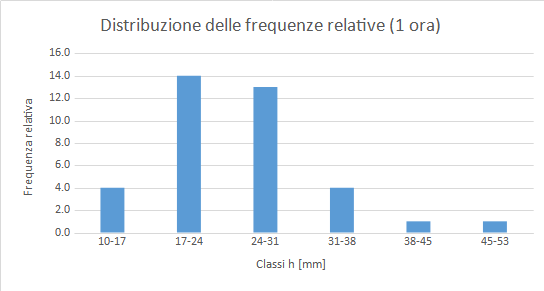
\includegraphics[scale=.6]{immagini/freq_piogg_rel_1ora.png}
    \caption{Distribuzione delle frequenze relative di pioggia (suddivise per classi omogenee), di un evento di durata 1 ora.}
  \label{freq_rel_piogg_05ore}
\end{figure}

\begin{figure}[H]\centering
    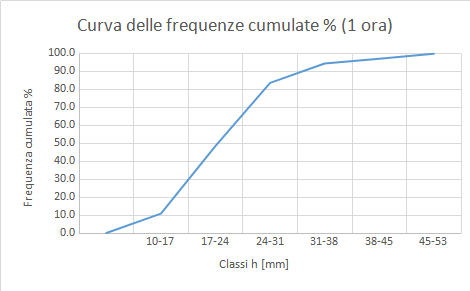
\includegraphics[scale=.6]{immagini/freq_piogg_cum_1ora.png}
    \caption{Frequenze di pioggia cumulata, relative ad un evento di durata 1 ora.}
  \label{freq_cum_piogg_05ore}
\end{figure}

\begin{table}[H] \centering
    \caption{\textcolor{red}{Valori di altezza di pioggia attesa (teorica), calcolata mediante la variabile d'appoggio $y$ di Weibull o di Hazen (1 ora).}}
    \begin{tabular}{cccc}
 & & \multicolumn{2}{c}{$h = Y/\alpha + u$}       \\
 \toprule
    \textbf{n} & \textbf{h (mm)  1 ora} & \textbf{h mediante Weibull} & \textbf{h mediante Hazen} \\
\midrule
    n         & h (mm)     1 ora & h\_calc Weib   & h\_calc Hazen  \\
    1         & 13.8             & 14.322         & 13.335         \\
    2         & 14.4             & 15.562         & 15.063         \\
    3         & 16.2             & 16.431         & 16.082         \\
    4         & 17               & 17.136         & 16.864         \\
    5         & 17.6             & 17.748         & 17.525         \\
    6         & 17.8             & 18.301         & 18.112         \\
    7         & 19.2             & 18.812         & 18.650         \\
    8         & 19.4             & 19.294         & 19.154         \\
    9         & 19.4             & 19.755         & 19.633         \\
    10        & 20.6             & 20.201         & 20.094         \\
    11        & 20.6             & 20.635         & 20.542         \\
    12        & 21.2             & 21.062         & 20.982         \\
    13        & 21.6             & 21.484         & 21.416         \\
    14        & 21.8             & 21.904         & 21.848         \\
    15        & 23.6             & 22.324         & 22.279         \\
    16        & 23.6             & 22.746         & 22.712         \\
    17        & 23.8             & 23.172         & 23.149         \\
    18        & 24               & 23.605         & 23.593         \\
    19        & 24.2             & 24.045         & 24.045         \\
    20        & 24.4             & 24.496         & 24.509         \\
    21        & 24.4             & 24.960         & 24.985         \\
    22        & 24.8             & 25.439         & 25.479         \\
    23        & 25.8             & 25.937         & 25.992         \\
    24        & 26.8             & 26.456         & 26.528         \\
    25        & 27               & 27.002         & 27.093         \\
    26        & 27.6             & 27.579         & 27.692         \\
    27        & 28               & 28.193         & 28.332         \\
    28        & 28.8             & 28.853         & 29.022         \\
    29        & 30.2             & 29.569         & 29.774         \\
    30        & 30.2             & 30.355         & 30.605         \\
    31        & 30.4             & 31.231         & 31.539         \\
    32        & 31.2             & 32.225         & 32.610         \\
    33        & 31.6             & 33.382         & 33.877         \\
    34        & 34.2             & 34.777         & 35.438         \\
    35        & 37.8             & 36.548         & 37.496         \\
    36        & 42.6             & 39.008         & 40.576         \\
    37        & 49.8             & 43.153         & 47.100         \\
    \bottomrule
    \end{tabular}
    \end{table}

\begin{figure}[H]\centering
        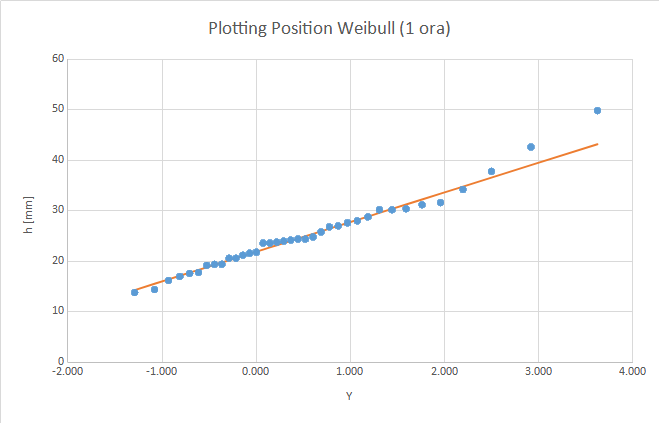
\includegraphics[scale=.5]{immagini/plot_pos_weib_1ora.png}
        \caption{Plotting position mediante Weibull (1 ora).}
      \label{plot_pos_weib_1ora}
 \end{figure}

\begin{figure}[H]\centering
        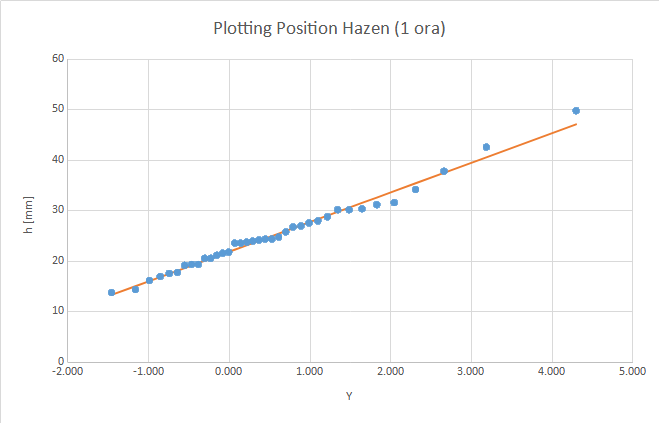
\includegraphics[scale=.5]{immagini/plot_pos_hazen_1ora.png}
        \caption{Plotting position mediante Hazen (1 ora).}
      \label{plot_pos_hazen_1ora}
\end{figure}

\begin{table}[H] \centering
    \caption{\textcolor{red}{Altezze di pioggia attese per il $T_r$ di riferimento e durata di 1 ora.}}
        \begin{tabular}{ccc}
        \toprule
        Tr (anni) & y     & h attesa (mm) \\
        \midrule
        2 & 0.367 & 24.0  \\
        5 & 1.500 & 30.7  \\
        10  & 2.250 & 35.1          \\
        30  & 3.384 & 41.7          \\
        50  & 3.902 & 44.8          \\
        100 & 4.600 & 48.9          \\
        200 & 5.296 & 53.0          \\         
        \bottomrule
        \end{tabular}
\end{table}

\begin{table}[H] \centering
    \caption{\textcolor{red}{Parametri per l'esecuzione del test statistico di Matalas, relativi alla durata di precipitazione di 1 ora.}}
    \begin{tabular}{cc}
    \toprule
    media                  & 25.28 \\
    $N ^{0.5}$             &  6.083\\
    G                      & 1.158 \\
    G - E                  &  0.277\\
    2 $\sigma$             & 1.069 \\
    TEST                   & Vero \\
    \bottomrule
    \end{tabular}
\end{table}

\subsubsection{Durata di 3 ore}
\begin{table}[H] \centering
    \caption{\textcolor{red}{Valori di probabilità di non superamento dell'evento (calcolata mediante Weibull e Hazen) e relativo valore del parametro d'appoggio $y$, riferito ad una durata di precipitazione di 3 ore.}}
\begin{tabular}{cccccc}
    &  & \multicolumn{2}{c}{\textbf{Plotting Position}} & \multicolumn{2}{c}{\textbf{Y -ln( -ln (1- 1/Tr))}}\\
    \toprule
       \textbf{n} & \textbf{h [mm] 1 ora} & \textbf{P Weibull   n/N+1} & \textbf{P Hazen  (n-0,5)/N} & \textbf{y Weibull} & \textbf{y Hazen}\\
   \midrule 
    1          & 18.6                      & 0.026                      & 0.014                       & -1.291                  & -1.460                  \\
    2          & 19.6                      & 0.053                      & 0.041                       & -1.080                  & -1.165                  \\
    3          & 21.8                      & 0.079                      & 0.068                       & -0.932                  & -0.991                  \\
    4          & 21.8                      & 0.105                      & 0.095                       & -0.812                  & -0.858                  \\
    5          & 23.4                      & 0.132                      & 0.122                       & -0.707                  & -0.745                  \\
    6          & 24.6                      & 0.158                      & 0.149                       & -0.613                  & -0.645                  \\
    7          & 24.8                      & 0.184                      & 0.176                       & -0.526                  & -0.553                  \\
    8          & 25.4                      & 0.211                      & 0.203                       & -0.443                  & -0.468                  \\
    9          & 26.8                      & 0.237                      & 0.230                       & -0.365                  & -0.386                  \\
    10         & 27.8                      & 0.263                      & 0.257                       & -0.289                  & -0.307                  \\
    11         & 28                        & 0.289                      & 0.284                       & -0.215                  & -0.231                  \\
    12         & 30.4                      & 0.316                      & 0.311                       & -0.142                  & -0.156                  \\
    13         & 30.4                      & 0.342                      & 0.338                       & -0.070                  & -0.082                  \\
    14         & 31.2                      & 0.368                      & 0.365                       & 0.001                   & -0.008                  \\
    15         & 31.8                      & 0.395                      & 0.392                       & 0.073                   & 0.065                   \\
    16         & 32.8                      & 0.421                      & 0.419                       & 0.145                   & 0.139                   \\
    17         & 33                        & 0.447                      & 0.446                       & 0.218                   & 0.214                   \\
    18         & 33.2                      & 0.474                      & 0.473                       & 0.291                   & 0.289                   \\
    19         & 33.2                      & 0.500                      & 0.500                       & 0.367                   & 0.367                   \\
    20         & 33.8                      & 0.526                      & 0.527                       & 0.443                   & 0.446                   \\
    21         & 34                        & 0.553                      & 0.554                       & 0.522                   & 0.527                   \\
    22         & 35.4                      & 0.579                      & 0.581                       & 0.604                   & 0.611                   \\
    23         & 35.8                      & 0.605                      & 0.608                       & 0.689                   & 0.698                   \\
    24         & 35.8                      & 0.632                      & 0.635                       & 0.778                   & 0.790                   \\
    25         & 35.8                      & 0.658                      & 0.662                       & 0.871                   & 0.886                   \\
    26         & 36                        & 0.684                      & 0.689                       & 0.969                   & 0.988                   \\
    27         & 36.2                      & 0.711                      & 0.716                       & 1.074                   & 1.097                   \\
    28         & 37.2                      & 0.737                      & 0.743                       & 1.186                   & 1.215                   \\
    29         & 38.2                      & 0.763                      & 0.770                       & 1.308                   & 1.343                   \\
    30         & 38.4                      & 0.789                      & 0.797                       & 1.442                   & 1.485                   \\
    31         & 41.4                      & 0.816                      & 0.824                       & 1.592                   & 1.644                   \\
    32         & 41.6                      & 0.842                      & 0.851                       & 1.761                   & 1.827                   \\
    33         & 44.8                      & 0.868                      & 0.878                       & 1.958                   & 2.043                   \\
    34         & 45.8                      & 0.895                      & 0.905                       & 2.196                   & 2.309                   \\
    35         & 46                        & 0.921                      & 0.932                       & 2.498                   & 2.660                   \\
    36         & 50.6                      & 0.947                      & 0.959                       & 2.918                   & 3.185                   \\
    37         & 75.4                      & 0.974                      & 0.986                       & 3.624                   & 4.297              \\
    \bottomrule    
    \end{tabular}
    \end{table}

\begin{table}[H] \centering
        \caption{\textcolor{red}{Principali parametri statistici riferiti alla serie pluviometrica di durata 3 ore.}}
     \begin{tabular}{cc}
        \toprule
    deviazione standard ($\sigma$) & 10.3 \\
    media ($x_m$)              & 34.1 \\
    $\alpha$            &  0.1 \\
    $u$           & 29.4\\
    N                & 37 \\
    minimo ($x_{min}$)      & 18.6 \\
    massimo ($x_{max}$)     & 75.4 \\
    varianza ($\sigma^2$)            & 106.7 \\
    coeff. variazione (CV)    &  0.3\\
    mediana ($x_{mediana}$)        & 33.2 \\
    numero di classi (k)      & 5.5  \\
    k scelto                 &  6.0 \\
    verifica (Iman e Conover) & 64.0 \\
    delta classe ($\Delta$)          & 9.5  \\
    delta scelto             & 10.0 \\
            \bottomrule
            \end{tabular}
    \end{table}

\begin{figure}[H]\centering
        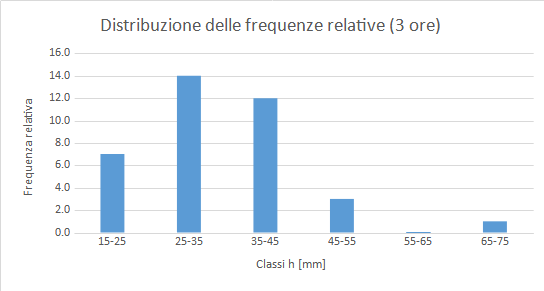
\includegraphics[scale=.6]{immagini/freq_piogg_rel_3ore.png}
        \caption{Distribuzione delle frequenze relative di pioggia (suddivise per classi omogenee), di un evento di durata 3 ore.}
      \label{freq_rel_piogg_05ore}
\end{figure}
    
\begin{figure}[H]\centering
        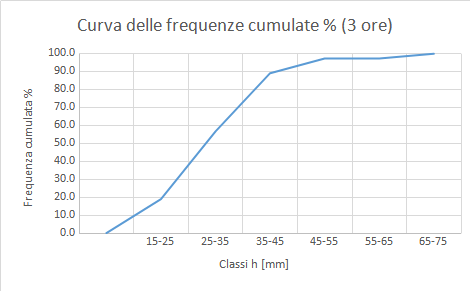
\includegraphics[scale=.6]{immagini/freq_piogg_cum_3ore.png}
        \caption{Frequenze di pioggia cumulata, relative ad un evento di durata 3 ore.}
      \label{freq_cum_piogg_05ore}
\end{figure}

\begin{table}[H] \centering
    \caption{\textcolor{red}{Valori di altezza di pioggia attesa (teorica), calcolata mediante la variabile d'appoggio $y$ di Weibull o di Hazen (3 ore).}}
    \begin{tabular}{cccc}
 & & \multicolumn{2}{c}{$h = Y/\alpha + u$}       \\
 \toprule
    \textbf{n} & \textbf{h (mm)  3 ore} & \textbf{h mediante Weibull} & \textbf{h mediante Hazen} \\
\midrule
    1          & 18.6                      & 19.035                & 17.681                 \\
    2          & 19.6                      & 20.737                & 20.053                 \\
    3          & 21.8                      & 21.929                & 21.450                 \\
    4          & 21.8                      & 22.897                & 22.524                 \\
    5          & 23.4                      & 23.738                & 23.431                 \\
    6          & 24.6                      & 24.496                & 24.237                 \\
    7          & 24.8                      & 25.198                & 24.975                 \\
    8          & 25.4                      & 25.860                & 25.666                 \\
    9          & 26.8                      & 26.492                & 26.324                 \\
    10         & 27.8                      & 27.104                & 26.957                 \\
    11         & 28                        & 27.700                & 27.572                 \\
    12         & 30.4                      & 28.286                & 28.176                 \\
    13         & 30.4                      & 28.865                & 28.771                 \\
    14         & 31.2                      & 29.441                & 29.364                 \\
    15         & 31.8                      & 30.018                & 29.955                 \\
    16         & 32.8                      & 30.597                & 30.550                 \\
    17         & 33                        & 31.182                & 31.150                 \\
    18         & 33.2                      & 31.775                & 31.759                 \\
    19         & 33.2                      & 32.380                & 32.380                 \\
    20         & 33.8                      & 32.999                & 33.016                 \\
    21         & 34                        & 33.635                & 33.670                 \\
    22         & 35.4                      & 34.293                & 34.347                 \\
    23         & 35.8                      & 34.975                & 35.051                 \\
    24         & 35.8                      & 35.688                & 35.787                 \\
    25         & 35.8                      & 36.437                & 36.562                 \\
    26         & 36                        & 37.229                & 37.384                 \\
    27         & 36.2                      & 38.072                & 38.262                 \\
    28         & 37.2                      & 38.978                & 39.209                 \\
    29         & 38.2                      & 39.960                & 40.241                 \\
    30         & 38.4                      & 41.039                & 41.382                 \\
    31         & 41.4                      & 42.241                & 42.663                 \\
    32         & 41.6                      & 43.606                & 44.134                 \\
    33         & 44.8                      & 45.194                & 45.872                 \\
    34         & 45.8                      & 47.108                & 48.015                 \\
    35         & 46                        & 49.538                & 50.840                 \\
    36         & 50.6                      & 52.914                & 55.066                 \\
    37         & 75.4                      & 58.603                & 64.020          \\
    \bottomrule      
    \end{tabular}
    \end{table}

    \begin{figure}[H]\centering
        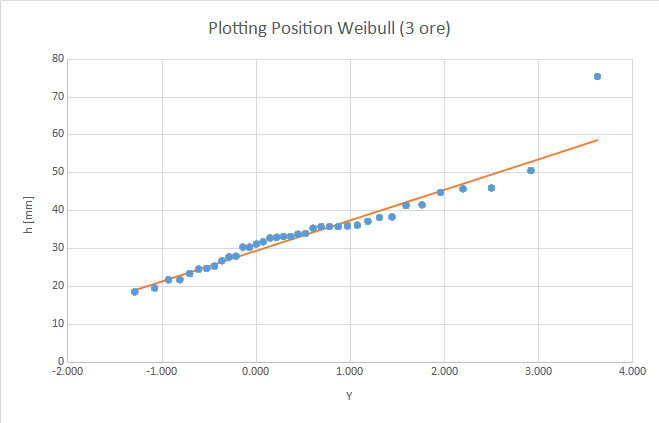
\includegraphics[scale=.5]{immagini/plot_pos_weib_3ore.png}
        \caption{Plotting position mediante Weibull (3 ore).}
      \label{plot_pos_weib_3ore}
 \end{figure}

\begin{figure}[H]\centering
        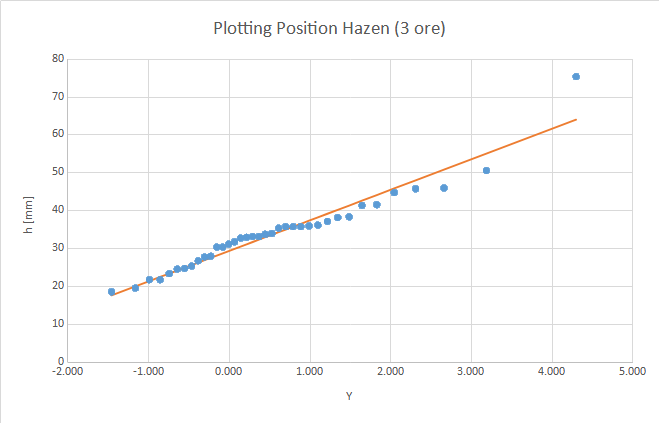
\includegraphics[scale=.5]{immagini/plot_pos_hazen_3ore.png}
        \caption{Plotting position mediante Hazen (3 ore).}
      \label{plot_pos_hazen_3ore}
\end{figure}

\begin{table}[H] \centering
    \caption{\textcolor{red}{Altezze di pioggia attese per il $T_r$ di riferimento e durata di 3 ore.}}
        \begin{tabular}{ccc}
        \toprule
        Tr (anni) & y     & h attesa (mm) \\
        \midrule
        2 & 0.367 & 32.4  \\
        5 & 1.500 & 41.5  \\
        10  & 2.250 & 47.5          \\
        30  & 3.384 & 56.7          \\
        50  & 3.902 & 60.8          \\
        100 & 4.600 & 66.5          \\
        200 & 5.296 & 72.1          \\         
        \bottomrule
        \end{tabular}
\end{table}

\begin{table}[H] \centering
    \caption{\textcolor{red}{Parametri per l'esecuzione del test statistico di Matalas, relativi alla durata di precipitazione di 3 ore.}}
    \begin{tabular}{cc}
    \toprule
    media                  & 34.08 \\
    $N ^{0.5}$             &  6.083\\
    G                      & 1.680 \\
    G - E                  &  0.799\\
    2 $\sigma$             & 1.069 \\
    TEST                   & Vero \\
    \bottomrule
    \end{tabular}
\end{table}

\subsubsection{Durata di 6 ore}
\begin{table}[H] \centering
    \caption{\textcolor{red}{Valori di probabilità di non superamento dell'evento (calcolata mediante Weibull e Hazen) e relativo valore del parametro d'appoggio $y$, riferito ad una durata di precipitazione di 6 ore.}}
\begin{tabular}{cccccc}
        &  & \multicolumn{2}{c}{\textbf{Plotting Position}} & \multicolumn{2}{c}{\textbf{Y -ln( -ln (1- 1/Tr))}}\\
        \toprule
           \textbf{n} & \textbf{h [mm] 1 ora} & \textbf{P Weibull   n/N+1} & \textbf{P Hazen  (n-0,5)/N} & \textbf{y Weibull} & \textbf{y Hazen}\\
       \midrule 
    1          & 25                          & 0.026                      & 0.014                       & -1.291                  & -1.460                  \\
    2          & 26.4                        & 0.053                      & 0.041                       & -1.080                  & -1.165                  \\
    3          & 26.8                        & 0.079                      & 0.068                       & -0.932                  & -0.991                  \\
    4          & 27.8                        & 0.105                      & 0.095                       & -0.812                  & -0.858                  \\
    5          & 30.4                        & 0.132                      & 0.122                       & -0.707                  & -0.745                  \\
    6          & 32.6                        & 0.158                      & 0.149                       & -0.613                  & -0.645                  \\
    7          & 32.8                        & 0.184                      & 0.176                       & -0.526                  & -0.553                  \\
    8          & 33                          & 0.211                      & 0.203                       & -0.443                  & -0.468                  \\
    9          & 33.6                        & 0.237                      & 0.230                       & -0.365                  & -0.386                  \\
    10         & 35.6                        & 0.263                      & 0.257                       & -0.289                  & -0.307                  \\
    11         & 37.2                        & 0.289                      & 0.284                       & -0.215                  & -0.231                  \\
    12         & 37.6                        & 0.316                      & 0.311                       & -0.142                  & -0.156                  \\
    13         & 37.8                        & 0.342                      & 0.338                       & -0.070                  & -0.082                  \\
    14         & 38.4                        & 0.368                      & 0.365                       & 0.001                   & -0.008                  \\
    15         & 39.4                        & 0.395                      & 0.392                       & 0.073                   & 0.065                   \\
    16         & 41.8                        & 0.421                      & 0.419                       & 0.145                   & 0.139                   \\
    17         & 41.8                        & 0.447                      & 0.446                       & 0.218                   & 0.214                   \\
    18         & 42.2                        & 0.474                      & 0.473                       & 0.291                   & 0.289                   \\
    19         & 42.6                        & 0.500                      & 0.500                       & 0.367                   & 0.367                   \\
    20         & 44.4                        & 0.526                      & 0.527                       & 0.443                   & 0.446                   \\
    21         & 44.8                        & 0.553                      & 0.554                       & 0.522                   & 0.527                   \\
    22         & 45                          & 0.579                      & 0.581                       & 0.604                   & 0.611                   \\
    23         & 46.6                        & 0.605                      & 0.608                       & 0.689                   & 0.698                   \\
    24         & 47.2                        & 0.632                      & 0.635                       & 0.778                   & 0.790                   \\
    25         & 48                          & 0.658                      & 0.662                       & 0.871                   & 0.886                   \\
    26         & 48.8                        & 0.684                      & 0.689                       & 0.969                   & 0.988                   \\
    27         & 50.6                        & 0.711                      & 0.716                       & 1.074                   & 1.097                   \\
    28         & 51.4                        & 0.737                      & 0.743                       & 1.186                   & 1.215                   \\
    29         & 51.4                        & 0.763                      & 0.770                       & 1.308                   & 1.343                   \\
    30         & 51.8                        & 0.789                      & 0.797                       & 1.442                   & 1.485                   \\
    31         & 52.8                        & 0.816                      & 0.824                       & 1.592                   & 1.644                   \\
    32         & 53.2                        & 0.842                      & 0.851                       & 1.761                   & 1.827                   \\
    33         & 55.6                        & 0.868                      & 0.878                       & 1.958                   & 2.043                   \\
    34         & 58.2                        & 0.895                      & 0.905                       & 2.196                   & 2.309                   \\
    35         & 65.4                        & 0.921                      & 0.932                       & 2.498                   & 2.660                   \\
    36         & 71.6                        & 0.947                      & 0.959                       & 2.918                   & 3.185                   \\
    37         & 130.2                       & 0.974                      & 0.986                       & 3.624                   & 4.297   \\
    \bottomrule               
    \end{tabular}
    \end{table}

\begin{table}[H] \centering
        \caption{\textcolor{red}{Principali parametri statistici riferiti alla serie pluviometrica di durata 6 ore.}}
     \begin{tabular}{cc}
        \toprule
    deviazione standard ($\sigma$) &  10.8\\
    media ($x_m$)              &  43.0\\
    $\alpha$            &  0.1 \\
    $u$           & 38.2\\
    N                &  37\\
    minimo ($x_{min}$)             & 25.0 \\
    massimo ($x_{max}$)            &  71.6\\
    varianza ($\sigma^2$)            &  117.7\\
    coeff. variazione (CV)    & 0.24 \\
    mediana ($x_{mediana}$)        &42.4  \\
    numero di classi (k)      &  5.4 \\
    k scelto                 &  6.0 \\
    verifica (Iman e Conover) &  64.0\\
    delta classe ($\Delta$)          & 7.8  \\
    delta scelto             & 8.0 \\
            \bottomrule
            \end{tabular}
    \end{table}

\begin{figure}[H]\centering
        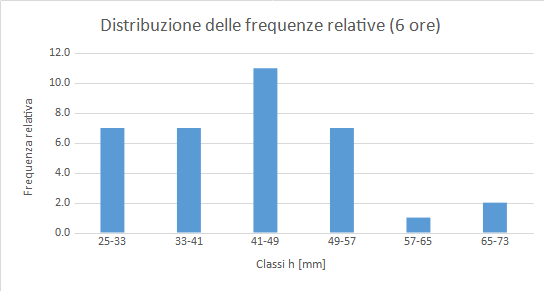
\includegraphics[scale=.6]{immagini/freq_piogg_rel_6ore.png}
        \caption{Distribuzione delle frequenze relative di pioggia (suddivise per classi omogenee), di un evento di durata 6 ore.}
      \label{freq_rel_piogg_05ore}
\end{figure}
    
\begin{figure}[H]\centering
        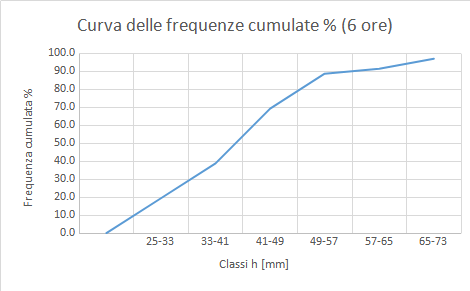
\includegraphics[scale=.6]{immagini/freq_piogg_cum_6ore.png}
        \caption{Frequenze di pioggia cumulata, relative ad un evento di durata 6 ore.}
      \label{freq_cum_piogg_05ore}
\end{figure}    

\begin{table}[H] \centering
    \caption{\textcolor{red}{Valori di altezza di pioggia attesa (teorica), calcolata mediante la variabile d'appoggio $y$ di Weibull o di Hazen (6 ore).}}
    \begin{tabular}{cccc}
 & & \multicolumn{2}{c}{$h = Y/\alpha + u$}       \\
 \toprule
    \textbf{n} & \textbf{h (mm)  6 ore} & \textbf{h mediante Weibull} & \textbf{h mediante Hazen} \\
\midrule
    1          & 25                          & 27.245                & 25.823                 \\
    2          & 26.4                        & 29.033                & 28.315                 \\
    3          & 26.8                        & 30.285                & 29.782                 \\
    4          & 27.8                        & 31.302                & 30.910                 \\
    5          & 30.4                        & 32.185                & 31.863                 \\
    6          & 32.6                        & 32.981                & 32.709                 \\
    7          & 32.8                        & 33.719                & 33.485                 \\
    8          & 33                          & 34.414                & 34.211                 \\
    9          & 33.6                        & 35.079                & 34.901                 \\
    10         & 35.6                        & 35.721                & 35.566                 \\
    11         & 37.2                        & 36.347                & 36.213                 \\
    12         & 37.6                        & 36.963                & 36.847                 \\
    13         & 37.8                        & 37.571                & 37.473                 \\
    14         & 38.4                        & 38.176                & 38.095                 \\
    15         & 39.4                        & 38.782                & 38.716                 \\
    16         & 41.8                        & 39.390                & 39.341                 \\
    17         & 41.8                        & 40.005                & 39.971                 \\
    18         & 42.2                        & 40.628                & 40.611                 \\
    19         & 42.6                        & 41.263                & 41.263                 \\
    20         & 44.4                        & 41.913                & 41.931                 \\
    21         & 44.8                        & 42.582                & 42.618                 \\
    22         & 45                          & 43.272                & 43.329                 \\
    23         & 46.6                        & 43.990                & 44.069                 \\
    24         & 47.2                        & 44.738                & 44.842                 \\
    25         & 48                          & 45.525                & 45.657                 \\
    26         & 48.8                        & 46.357                & 46.520                 \\
    27         & 50.6                        & 47.242                & 47.442                 \\
    28         & 51.4                        & 48.194                & 48.437                 \\
    29         & 51.4                        & 49.226                & 49.521                 \\
    30         & 51.8                        & 50.359                & 50.719                 \\
    31         & 52.8                        & 51.622                & 52.065                 \\
    32         & 53.2                        & 53.055                & 53.610                 \\
    33         & 55.6                        & 54.723                & 55.436                 \\
    34         & 58.2                        & 56.734                & 57.687                 \\
    35         & 65.4                        & 59.287                & 60.654                 \\
    36         & 71.6                        & 62.833                & 65.093                 \\
    37         & 130.2                       & 68.809                & 74.499       \\
    \bottomrule         
    \end{tabular}
    \end{table}

\begin{figure}[H]\centering
        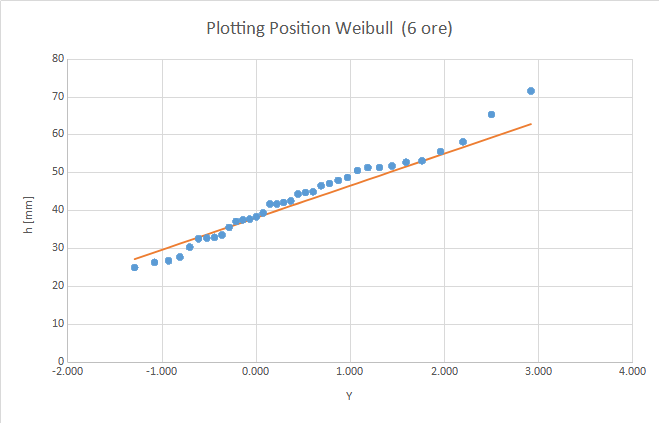
\includegraphics[scale=.5]{immagini/plot_pos_weib_6ore.png}
        \caption{Plotting position mediante Weibull (6 ore).}
      \label{plot_pos_weib_6ore}
 \end{figure}

\begin{figure}[H]\centering
        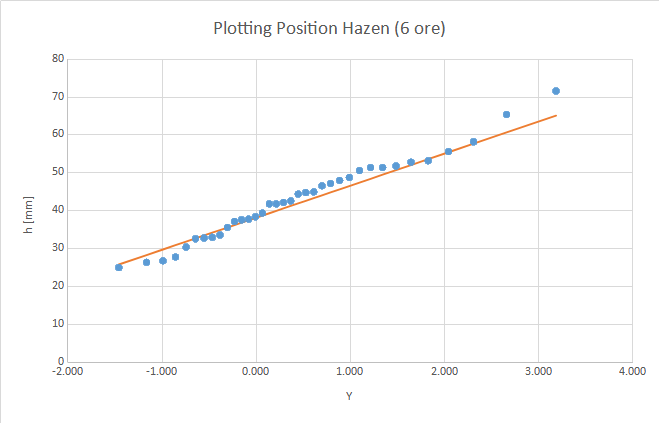
\includegraphics[scale=.5]{immagini/plot_pos_hazen_6ore.png}
        \caption{Plotting position mediante Hazen (6 ore).}
      \label{plot_pos_hazen_6ore}
\end{figure}

\begin{table}[H] \centering
    \caption{\textcolor{red}{Altezze di pioggia attese per il $T_r$ di riferimento e durata di 6 ore.}}
        \begin{tabular}{ccc}
        \toprule
        Tr (anni) & y     & h attesa (mm) \\
        \midrule
        2 & 0.367 & 41.3  \\
        5 & 1.500 & 50.8  \\
        10  & 2.250 & 57.2          \\
        30  & 3.384 & 66.8          \\
        50  & 3.902 & 71.2          \\
        100 & 4.600 & 77.1          \\
        200 & 5.296 & 82.9          \\         
        \bottomrule
        \end{tabular}
\end{table}

\begin{table}[H] \centering
    \caption{\textcolor{red}{Parametri per l'esecuzione del test statistico di Matalas, relativi alla durata di precipitazione di 6 ore.}}
    \begin{tabular}{cc}
    \toprule
    media                  & 43.04 \\
    $N ^{0.5}$             &  6.000\\
    G                      & 0.434 \\
    G - E                  &  0.447\\
    2 $\sigma$             & 1.069 \\
    TEST                   & Vero \\
    \bottomrule
    \end{tabular}
\end{table}

\subsection{LSPP - Linee segnalatrici di probabilità pluviometrica}
Dopo aver ottenuto le quantità di precipitazioni teoriche, per ogni durata di evento pluviometrico e per diversi tempi di ritorno, è possibile creare un grafico che metta in relazione tutti questi parametri.

\begin{table}[H]\centering
    \caption{\textcolor{red}{Tabella riassuntiva delle altezze di pioggia previste per determinate durate e per determinati tempi di ritorno.}}
    \begin{tabular}{ccccccc}
    \toprule
    \multirow{2}{*}{\textbf{durata t (ore)}} & \multicolumn{6}{c}{\textbf{Altezza di pioggia attesa h (mm) per Tr}} \\
  & \textbf{2 anni} & \textbf{5 anni} & \textbf{30 anni} & \textbf{50 anni} & \textbf{100 anni} & \textbf{200 anni} \\
    \textbf{0.5}                             & 19.83           & 25.30           & 34.38            & 36.88            & 40.25             & 43.60             \\
    \textbf{1}                               & 24.05           & 30.69           & 41.75            & 44.78            & 48.88             & 52.96             \\
    \textbf{3}                               & 32.38           & 41.50           & 56.67            & 60.84            & 66.46             & 72.06             \\
    \textbf{6}                               & 41.26           & 50.85           & 66.78            & 71.16            & 77.06             & 82.94            \\
    \bottomrule
    \end{tabular}
    \label{figure:altezze_critiche_pioggia}
    \end{table}

La curva interpolatrice ha un andamento caratteristico che segue la funzione $h=at^n$, con $a$ che dipende dal tempo di ritorno T e con $n$ che risulta essere una costante per la stazione di rilevamento dei dati (in Italia generalmente è tra 0.20 e 0.55). Il parametro $n$ è un valore sempre inferiore ad 1 perchè all'aumentare del tempo dell'evento pluviometrico, l'intensità di pioggia cala.\\
Essendo che:
\begin{equation}
    h=at^n \rightarrow \log h = \log a + n \log t \rightarrow H=A+nT
    \label{eq:formula_LSPP}
\end{equation}
Mediante l'equazione $H = \log h$, possiamo calcolare il valore di H della tabella \eqref{figure:altezze_critiche_pioggia}:

\begin{table}[H] \centering
    \caption{\textcolor{red}{Tabella riassuntiva delle altezze di pioggia previste per determinate durate e per determinati tempi di ritorno, in scala logaritmica.}}
    \begin{tabular}{ccccccc}
        \toprule
    \multirow{2}{*}{\textbf{T}} & \multicolumn{6}{c}{\textit{\textbf{H = log h}}}                                                            \\ & \textbf{2 anni} & \textbf{5 anni} & \textbf{30 anni} & \textbf{50 anni} & \textbf{100 anni} & \textbf{200 anni} \\
    \textbf{-0.301}             & 1.297           & 1.403           & 1.536            & 1.567            & 1.605             & 1.639             \\
    \textbf{0.000}              & 1.381           & 1.487           & 1.621            & 1.651            & 1.689             & 1.724             \\
    \textbf{0.477}              & 1.510           & 1.618           & 1.753            & 1.784            & 1.823             & 1.858             \\
    \textbf{0.778}              & 1.616           & 1.706           & 1.825            & 1.852            & 1.887             & 1.919  \\
    \bottomrule          
    \end{tabular}
    \end{table}
Nel caso in cui gli assi del grafico avessero entrambi la scala logaritmica, la linea interpolatrice dei punti sarebbe una retta.\\
Invertendo la formula della LSPP \eqref{eq:formula_LSPP}, è possibile calcolarsi i valori dei rimanenti parametri \eqref{table:valori_riassuntivi_lspp}.
\begin{table}[H] \centering
    \begin{tabular}{ccccccc}
    \toprule
 & \textbf{2 anni} & \textbf{5 anni} & \textbf{30 anni} & \textbf{50 anni} & \textbf{100 anni} & \textbf{200 anni} \\
    \textit{A} & 1.382  & 1.487  & 1.620  & 1.650  & 1.688  & 1.722  \\
    \textit{a} & 24.080 & 30.679 & 41.647 & 44.659 & 48.722 & 52.771 \\
    \textit{n} & 0.291  & 0.280  & 0.269  & 0.267  & 0.264  & 0.262  \\
    \bottomrule
    \end{tabular}
    \label{table:valori_riassuntivi_lspp}
    \end{table}
Riassumendo, le equazioni delle LSPP per la nostra area di studio, possiedono i parametri numerici \eqref{table:riassunto_lspp}.

\begin{table}[H] \centering
    \caption{\textcolor{red}{Parametri a e n per poter ricavare la funzione LSPP, dato un certo tempo di ritorno e di durata di pioggia.}}
    \begin{tabular}{ccc}
    \toprule
    \multirow{2}{*}{\textbf{Tempo di ritorno (anni)}} & \multicolumn{2}{c}{\textbf{LSPP}} \\
     & \textbf{a}      & \textbf{n}      \\
    2                                                 & 24.080          & 0.291           \\
    5                                                 & 30.679          & 0.280           \\
    30                                                & 41.647          & 0.269           \\
    50                                                & 44.659          & 0.267           \\
    100                                               & 48.722          & 0.264           \\
    200                                               & 52.771          & 0.262   \\
    \bottomrule  
    \label{parametri_LSPP}     
    \end{tabular}
    \label{table:riassunto_lspp}
    \end{table}

Per le durate di precipitazione già studiate in questa relazione (0.5, 1, 3 e 6 ore), la LSPP attribuisce le seguenti altezze di pioggia \eqref{table:altezze_ricavate_lspp}.

\begin{table}[H]\centering
    \caption{\textcolor{red}{Calcolo per le principali durate temporali dell'altezza di precipitazione prevista per un dato tempo di ritorno (mediante l'equazione LSPP).}}
    \begin{tabular}{ccccccc}
        \toprule
    \multirow{2}{*}{\textbf{$T_p$ (ore)}} & \multicolumn{6}{c}{\textit{\textbf{h calcolata (mm)}}}  \\
    & \textbf{Tr=2anni} & \textbf{Tr=5anni} & \textbf{Tr=30anni} & \textbf{Tr=50anni} & \textbf{Tr=100anni} & \textbf{Tr=200anni} \\
    \textbf{0.5}                           & 19.68                & 25.27                & 34.56                 & 37.12                 & 40.56                  & 44.00                  \\
    \textbf{1}                             & 24.08                & 30.68                & 41.65                 & 44.66                 & 48.72                  & 52.77                  \\
    \textbf{3}                             & 33.15                & 41.72                & 55.96                 & 59.87                 & 65.14                  & 70.40                  \\
    \textbf{6}                             & 40.55                & 50.66                & 67.43                 & 72.04                 & 78.25                  & 84.43           \\
    \bottomrule      
    \end{tabular}
    \label{table:altezze_ricavate_lspp}
    \end{table}

Conoscendo i parametri delle funzioni matematiche delle LSPP, è possibile vedere graficamente l'andamento di tali curve, creando un apposito grafico \eqref{figure:LSPP}.

\begin{figure}[H]\centering
        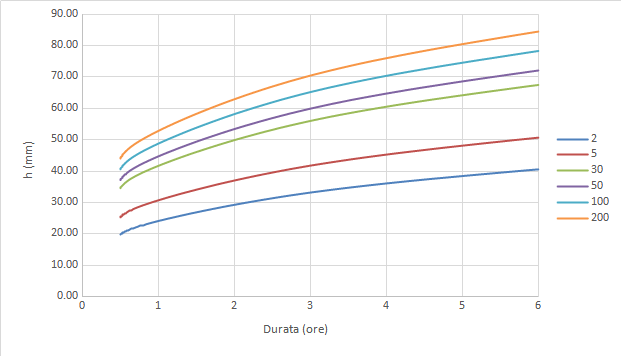
\includegraphics[scale=.75]{immagini/LSPP.png}
        \caption{Grafico della LSPP per ogni tempo di ritorno studiato, in anni.}
      \label{figure:LSPP}
\end{figure}

